\section{Annotation des sections et entités judiciaires}

\subsection{Objectif de la tâche}
\begin{frame}[t]{\mysubsectiontitle}
	Détecter les méta-données de référence et les normes utilisées
\begin{figure}
	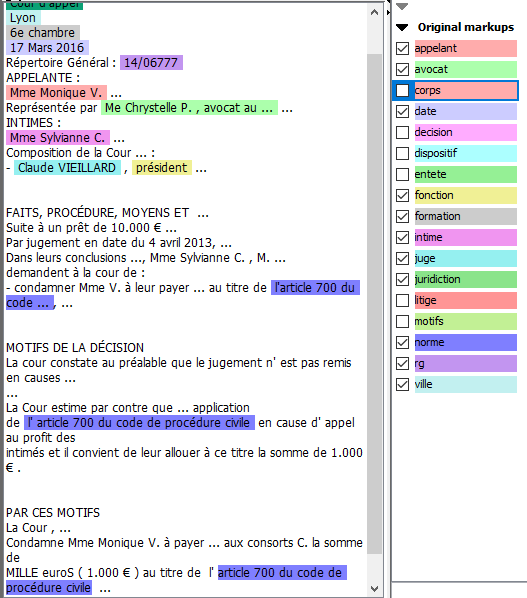
\includegraphics[height=\textheight]{decision-marquee.png}
\end{figure}
\end{frame}

\begin{frame}[t]{\mysubsectiontitle}
Sectionner pour organiser l'extraction des connaissances
\tiny
\begin{columns}\tiny
	\begin{column}{.45\linewidth}
		\fbox{\begin{minipage}{\textwidth}ARRÊT N°
				
				R.G: \textcolor{red}{11/03924}
				
				\textcolor{red}{COUR D'APPEL} DE \textcolor{red}{NÎMES}
				
				\textcolor{red}{CHAMBRE CIVILE}
				
				\textcolor{red}{1ère Chambre A}
				
				ARRÊT DU \textcolor{red}{20 MARS 2012}
				
				APPELANTE:
				
				\textcolor{red}{Madame Michéle A.} ...
				
				assistée de la \textcolor{red}{SELARL VAJOU}, ...
				
				INTIMES:
				
				\textcolor{red}{Monsieur Martial B} ...
				
				assisté de la \textcolor{red}{SCP MARION GUIZARD PATRICIA SERVAIS}, ...
				
				COMPOSITION DE LA COUR LORS DU DÉLIBÉRÉ:
				
				\textcolor{red}{M. Dominique BRUZY, Président}
				
				\textcolor{red}{M. Serge BERTHET, Conseiller}
				
				...
		\end{minipage}}
		\vspace{0.1cm}
		
		{\textbf{Entêtes}: méta-données}
	\end{column}
	\begin{column}{.55\linewidth}
		\fbox{\begin{minipage}{\textwidth}FAITS, PROCEDURE, ...
				
				Madame Michèle A. demande:
				
				...
				
				- de condamner Madame JONES-B. à lui payer la somme de \textcolor{red}{2.500 euros} au titre de l'\textcolor{red}{article 700 du Code de Procédure Civile}, 
		\end{minipage}}
		\vspace{0.1cm}
		
		{\textbf{Corps}: demandes, arguments et normes }
		
		\vspace{0.4cm}
		
		\fbox{\begin{minipage}{\textwidth}PAR CES MOTIFS, LA COUR:
				
				...
				
				Vu l'\textcolor{red}{article 809 du Code de Procédure Civile},
				
				...
				
				\textcolor{red}{Déboute Madame A. de sa demande de provision sur dommages-intérêts.}
				
				...
				
				Vu l'\textcolor{red}{article 700 du Code de Procédure Civile},
				
				Condamne Madame JONES-B. à verser à Madame A. la somme de \textcolor{red}{2.500 euros}.
		\end{minipage}}
		\vspace{0.1cm}
		
		{\textbf{Dispositif}: résultats et normes}
		
	\end{column}
\end{columns}
\end{frame}

\subsection{Approches probabilistes de détection d'entités}
\begin{frame}[t]{\mysubsectiontitle}
Modèles probabilistes à états et observations

\scriptsize
\begin{table}[]%width=\linewidth
%\begin{tabular}[]{p{0.40\linewidth}|p{0.55\linewidth}}
\begin{tabular}[]{c|c}
\toprule
{\textbf{HMM}} & {\textbf{CRF}} \\
%		\midrule
%		\textbf{Generative} models 	& \multicolumn{2}{c}{"\textbf{Discriminative}" or "\textbf{Conditional}" models } \\[0.25em]
%\midrule		
%"\textbf{generate}" input	& {"\textbf{condition}" on input }\\%[0.25em]
\midrule
{un seul descripteur  par observation}	& {plusieurs descripteurs complexes par observation}\\%[0.25em]
\midrule	
\begin{tikzpicture}[->,>=stealth',shorten >=1pt,auto,node distance=1.3cm,
semithick]
\node[state] (S1)                    {$s_{t-1}$};
\node[state]         (S2) [right of=S1] 	  {$s_{t}$};
\node[state]         (O) [below of=S2] {$o_{t}$};
\path (S1) edge              node {} (S2)
(S2) edge              node {} (O);
\end{tikzpicture}
& 

\begin{tikzpicture}[auto,>=stealth',shorten >=1pt,auto,node distance=1.3cm,
semithick]
\node[state] (S1)                    {$s_{t-1}$};
\node[state]         (S2) [right of=S1] 	  {$s_{t}$};
\node[state]         (O) [below of=S2] {$o_{t}$};
\path (S1) edge              node {} (S2)
(S2) edge              node {} (O);
\end{tikzpicture}					
\\%[0.25em]
\midrule
$P(S,O) = \prod\limits_{t=1}^{T} P(s_t \vert s_{t-1}) P(o_t \vert s_{t})$  & $P_\lambda(S|O) = \frac{1}{Z(O)}exp\left( \sum\limits_{t=1}^{T}\sum\limits_{k} \lambda_k f_k(s_{t-1},s_t, o_t) \right) $ \\
% & & & \\
\tiny \cite{Seymore1999hmm} & \tiny \cite{peng2006crf} \\ 
\bottomrule
\end{tabular}
\end{table}

\normalsize

Objectif: Trouver la séquence la plus probable d'étiquetage pour l'ensemble du texte

\textbf{Entrainement sur des séquences préalablement étiquetées}
\end{frame}

\subsection{Sélection de modèle}
\begin{frame}[t]{\mysubsectiontitle}		
	Méthodes explorées
	\begin{itemize} \scriptsize
		\item Descripteurs de lignes pour les sections : longueur ? position ? etc.
		\item Descripteurs de mots pour les entités : est-ce une initiale ("B.") ? est-ce un mot clé de citation de loi ? etc.
		\item Schéma d'étiquetage : distinction des parties d'une entité \tiny
		\begin{tabular}{l|ccccccccc}
			& \textit{composée} & \textit{de} & \textit{Madame} & \textit{Martine} & \textit{JEAN} & , & \textit{Président} & \textit{de} & ... \\ 
			IO & O & O & I-JUGE & I-JUGE & I-JUGE & O & I-FONCTION & I-FONCTION & ... \\
			BIO & O & O & B-JUGE & I-JUGE & I-JUGE & O & B-FONCTION & I-FONCTION & ... \\
			IEO & O & O & I-JUGE & I-JUGE & E-JUGE & O & I-FONCTION & I-FONCTION & ...\\
			BIEO & O & O & B-JUGE & I-JUGE & E-JUGE & O & B-FONCTION & I-FONCTION & ... \\
		\end{tabular}
		\item \scriptsize sélection du sous-ensemble de descripteurs court et aux meilleurs résultat (recherche par BDS et SFFS)
	\end{itemize}	
\end{frame}

\begin{frame}[t]{\mysubsectiontitle}
	Résultats (CRF)
\begin{figure}
	\begin{itemize}
		\item sélection du schéma d'étiquetage
		\begin{itemize}
			\item Les schémas plus complexes que IO rendent l'entraînement plus long
			\item Les schémas complexes ne semblent pas améliorer la détection des sections(baisse de $F_1$ de près de $20\%$)
			\item Les schémas complexes améliorent légèrement la détection d'entité de moins de $3\%$
		\end{itemize}
		\item sélection des descripteurs
		\begin{itemize}
			\item Lenteur des algorithmes BDS et SFFS (plus de 15h)
			\item BDS réduit de moitié
			\item SFFS réduit beaucoup plus
			\item Pas d'amélioration ou détérioration considérable de la détection
		\end{itemize}
	\end{itemize}
\end{figure}
\end{frame}

\subsection{Discussions des résultats}
\begin{frame}[t]{\mysubsectiontitle}
	Confusions de labels
\begin{figure}[!htb]
	\centering
	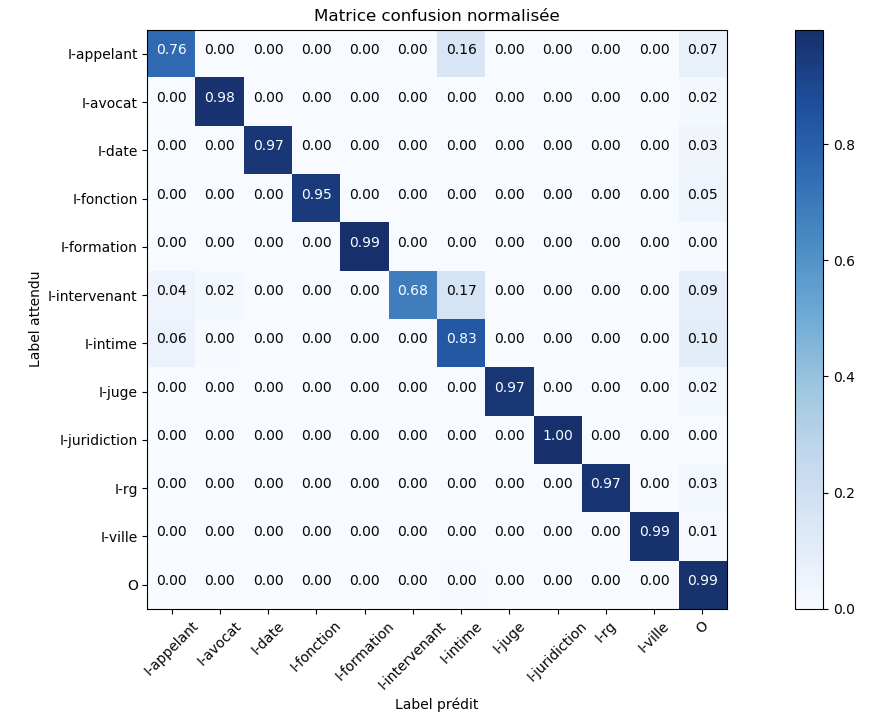
\includegraphics[width=0.6\textwidth]{confusion_matrix_entete.png} \hfill
	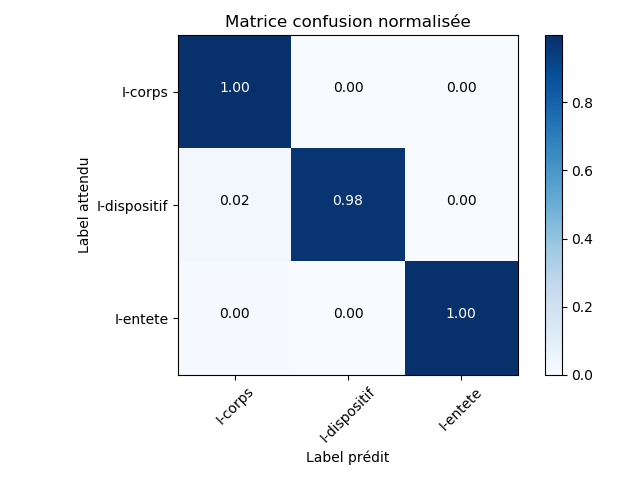
\includegraphics[width=0.38\textwidth]{confusion_matrix_section.png}
	%\textcolor{red}{Matrices de confusion}
	\caption{Matrice de confusion des modèles basés CRF}
	\label{fig:structuration:matrice-confusion-entete}
\end{figure}
\end{frame}

\begin{frame}[t]{\mysubsectiontitle}
	Impact de la quantité de décisions d'entraînement
\begin{figure}[!h]
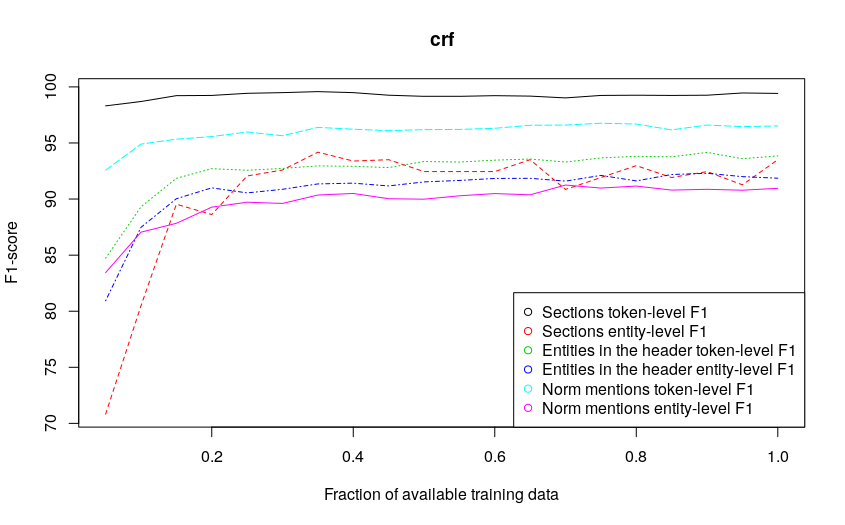
\includegraphics[width=0.9\textwidth]{lc-crf.png}
\caption{Evolution de la F1-mesure en fonction de la fraction utilisée}\label{p4_crf-learning-curves}
\end{figure}
\end{frame}

\begin{frame}[t]{\mysubsectiontitle}
	Description manuelle vs. représentation apprise
\scriptsize
\begin{tabular}{|l|l|l|l|l|l|l|}
	\hline
	&               \multicolumn{3}{c}{\textbf{CRF + descripteurs manuels}} & \multicolumn{3}{|c|}{\textbf{BiLSTM-CRF}}   \\ \cline{2-7}
	& \textit{Precision} & \textit{Rappel}                     & $F_1$ & \textit{Precision} & \textit{Rappel}      & $F_1$ \\ \hline
	\textbf{appelant}      & 82.49              & 69.42                               & 74.72       & 80.26              & 71.53                & 75.04       \\ 
	\textbf{avocat}        & 90.15              & 89.02                               & 89.56       & 84.93              & 87.88                & 86.36       \\ 
	\textbf{date}          & 95.34              & 91.46                               & 93.12       & 95.04              & 90.79                & 92.63       \\ 
	\textbf{fonction}      & 95.87              & 95.08                               & 95.44       & 92.69              & 93.48                & 93.03       \\ 
	\textbf{formation}     & 96.91              & 91.31                               & 93.7        & 91.05              & 89.47                & 89.84       \\ 
	\textbf{intervenant}   & 51.42              & 32.71                               & 36.8        & 31.48              & 20                   & 23.11       \\ 
	\textbf{intime}        & 76.01              & 79.15                               & 77.22       & 67.7               & 75.43                & 70.83       \\ 
	\textbf{juge}          & 95.67              & 94.07                               & 94.84       & 95.44              & 95.56                & 95.46       \\ 
	\textbf{juridiction}   & 98.55              & 98.25                               & 98.33       & 97.95              & 99.22                & 98.57       \\ 
	\textbf{rg}            & 95.46              & 95.29                               & 95.27       & 91.13              & 97.26                & 93.92       \\ 
	\textbf{ville}         & 98.33              & 93.01                               & 94.71       & 91.43              & 95.34                & 93.3        \\ 
	\textbf{norme}         & 91.08              & 90.27                               & 90.67       & 91.43              & 92.65                & 92.03       \\ \hline
	\noalign{\smallskip}\hline\noalign{\smallskip}
	\textbf{Evaluation globale} & 92.2               & 90.09                               & 91.12       & 89.21              & 90.43                & 89.81       \\ \hline
\end{tabular}
\end{frame}
